% !TEX root = template.tex

%----------------------------------------------------------------------
\section{Description / Strategy}

A Skiplist is basically a collection of sorted list nodes, where each node has a link to one or more following nodes. These links form shortcuts which can be used to speed up the searching by skipping one or more nodes. In contrast to tree-based search structures Skiplists don't require re-balancing, thus making the concurrent implementation easier.

%% TODO add more



%----------------------------------------------------------------------
\section{Implementation}

Each concrete Skiplist implements the \texttt{SkipList<T>} interface shown in Listing \ref{lst:skiplist_interface}, providing methods for inserting, removing and searching of values.

\begin{lstlisting}[language=C++, caption={Skiplist Interface}, label=lst:skiplist_interface]
template <typename T>
class SkipList
{
  public:
    static_assert(std::is_integral<T>::value, 
                  "T must be an integral type");
    
    virtual bool empty() = 0;
    virtual size_type size() = 0;
    virtual bool insert(const_reference value) = 0;
    virtual bool remove(const_reference value) = 0;
    virtual bool contains(const_reference value) = 0;
    virtual void clear() = 0;
};
\end{lstlisting}
\noindent For simplicity all the implementations only support integral types and can only handle unique values, meaning that adding the same value twice will fail on the second time. Additionally each type must have a specified minimum and maximum value, because these values will be used by the \texttt{head} and \texttt{tail} nodes respectively. 



%------------------
\subsection{Sequential}
The sequential Skiplist implements the algorithm described in TODO REF with two small optimizations. The current maximum level of all inserted nodes is cached so that the unused levels can be skipped immediately. Additionally the next-node pointers are stored in a static array within the node object itself, thus eliminating one indirection which would occur when using a dynamic datastructure such as \texttt{std::vector}, with the small downside that it always allocates \texttt{MaxHeight} next-pointer slots even if some slots are unused.

%------------------
\subsection{Concurrent}
The ConcurrentSkiplist is based on the sequential one and uses a \texttt{std::mutex} to control the concurrent access of multiple threads. The implementation simply forwards all requests to the internal instance of a sequential Skiplist after successfully grabbing the lock, i.e. the access to the internal sequential list is serialized.

%------------------
\subsection{Lazy}
The LazySkipList was based on the algorithm discussed in \cite{}. Instead of serializing all accesses as in the ConcurrentSkipList, it uses a \texttt{std::mutex} per node to serialize as little as possible.

\subsubsection*{Linearizability}
Additionally to the lock, each node contains two flags: \texttt{marked}, indicating that the node is virtually removed from the list and \texttt{fullyLinked}, which is set when the node is fully linked into the SkipList. These flags determine when a performed action (insert or remove) is visible to the other processes and therefore the moment when either the flag \texttt{marked} or \texttt{fullyLinked} is set to \texttt{true} is the linearization point of the respective method.

\subsubsection*{Memory-Managed Version}
In the standard implementations of the LazySkipList (and the LockFreeSkipList) the memory of nodes which are removed from the list is not deallocated. To fix this flaw, the MMLazySkipList uses \texttt{C++11} reference counted smart pointers to deallocate all removed nodes.

%------------------
\subsection{Lock-Free}
The LockFreeSkipList enables concurrent access without locks by using atomic \texttt{compareAndSet} operations for all list manipulations. Any list manipulations in the algorithm consists of changing the successor reference of a node while ensuring that the marked flag \textbf{and} the successor have not changed before. Because standard \texttt{compareAndSet} implementations only support to compare one value, we merge the reference and the marked flag into one \texttt{std::atomic\_uintptr\_t} by using one unused bit of the reference for our marked flag (See Listing \ref{lst:atomic_markable_reference}).

\begin{lstlisting}[language=C++, caption={AtomicMarkableReference}, label=lst:atomic_markable_reference]
template <typename T>
class AtomicMarkableReference
{
  public:
    AtomicMarkableReference(T* ref = nullptr, bool marked = false)
    {
        value = ((uintptr_t)ref & ~mask) | (marked ? 1 : 0);
    }

    T* get(bool& marked)
    {
        uintptr_t tmp = value;
        marked = (bool)(tmp & mask);
        return (T*)(tmp & ~mask);
    }

    bool compareAndSet(T* oldRef, T* newRef, bool oldMarked, bool newMarked)
    {
        uintptr_t oldValue = ((uintptr_t)oldRef & ~mask) | (oldMarked ? 1 : 0);
        uintptr_t newValue = ((uintptr_t)newRef & ~mask) | (newMarked ? 1 : 0);
        return value.compare_exchange_strong(oldValue, newValue);
    }

  private:
    std::atomic_uintptr_t value;
    static const uintptr_t mask = 1;
};
\end{lstlisting}

\subsubsection*{Linearizability}
\noindent As in the LazySkipList the linearization point for removing a list element is the moment when the marked flag is set to \texttt{true}. The linearization point for the insert operation is defined in the LockFreeSkipList as the moment the node is linked in at the bottom level.

%----------------------------------------------------------------------
\section{Experimental Setup}

%------------------
\subsection{Simulated Workloads}

\subsubsection{Interleaving Insert}

\subsubsection{Interleaving Remove}

\subsubsection{Mix of Insertions, Removals and Searches}


%------------------
\subsection{Skiplist Statistics}
To get a better picture about the performance and behavior of the Skiplist, performance counters have been added to the \texttt{insert}, \texttt{remove} and \texttt{contains} methods of all Skiplist implementations. These performance counters collect the number of retries, which is especially interesting for the lazy and lock free implementations, as well as the number of successful and failed invocations. Based on these performance counters multiple different metrics can be evaluated, such as the average number of retries of \texttt{insert}, \texttt{remove} and \texttt{contains}.\\

\noindent To minimize the possible influences on the benchmarking results, each thread collects the data in a thread-local statistics object, thus no locking and no atomics are required. At the end of each benchmark the thread-local statistics are aggregated by the benchmark suite to get the complete statistics.\\

\noindent The statistics collection can be completely turned off and thus doesn't add any overhead to production use.

%----------------------------------------------------------------------
\section{Experimental Results}

Each benchmark was repeated $30$ times. The execution time and Skiplist statistics of each repetition was collected and post-processed.

\subsection{Throughput}

\begin{figure}[H]
    \centering
    
    \begin{subfigure}[b]{0.49\textwidth}
        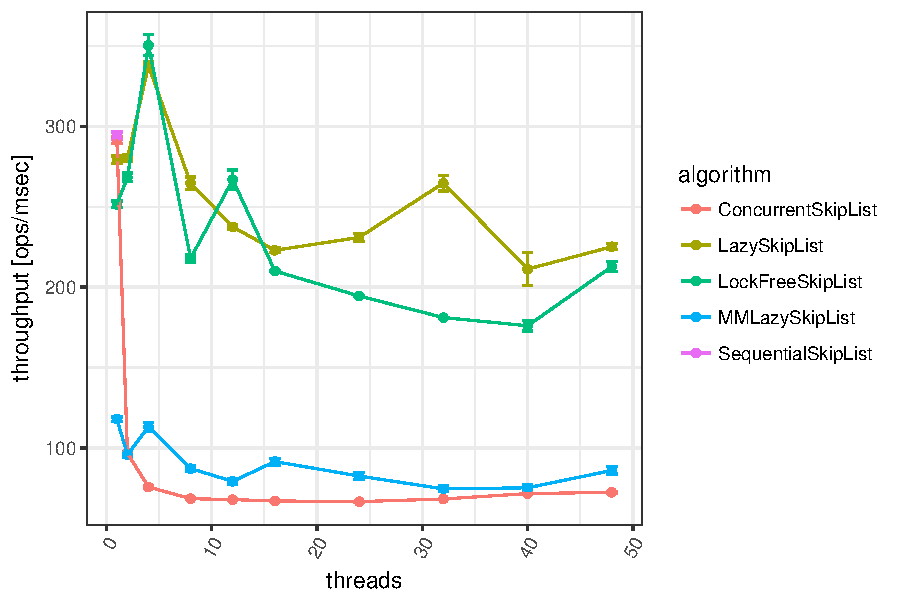
\includegraphics[width=\textwidth]{../plots/interleaving_insert_-_no_failed_inserts_strong_0.pdf}
        \caption{Interleaving Insert}
        \label{fig:Scatter:OpenMPI:Rel:31}
    \end{subfigure}
    \begin{subfigure}[b]{0.49\textwidth}
        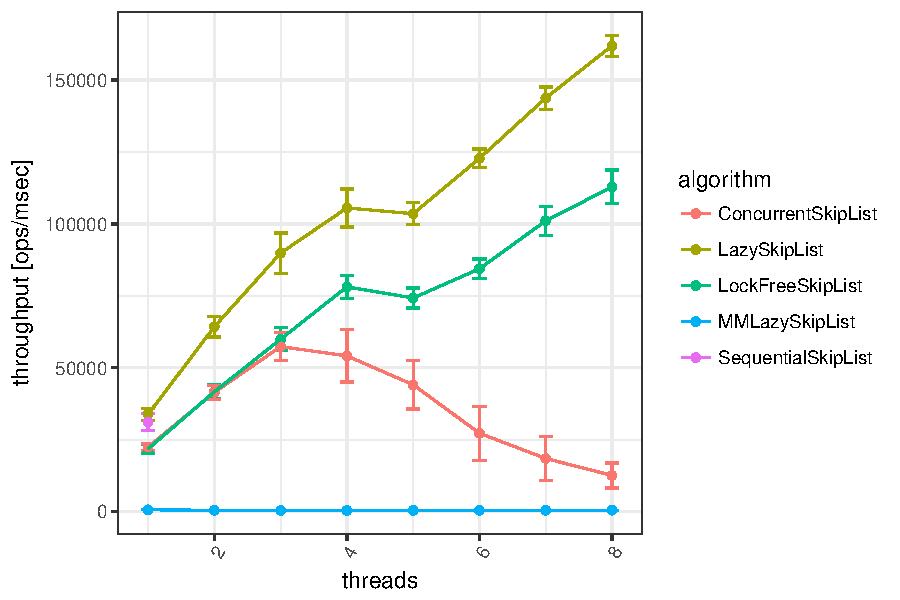
\includegraphics[width=\textwidth]{../plots/interleaving_remove_-_no_failed_removes_strong_0.pdf}
        \caption{Interleaving Remove}
        \label{fig:Scatter:OpenMPI:Abs:31}
    \end{subfigure}
    
    \begin{subfigure}[b]{0.49\textwidth}
        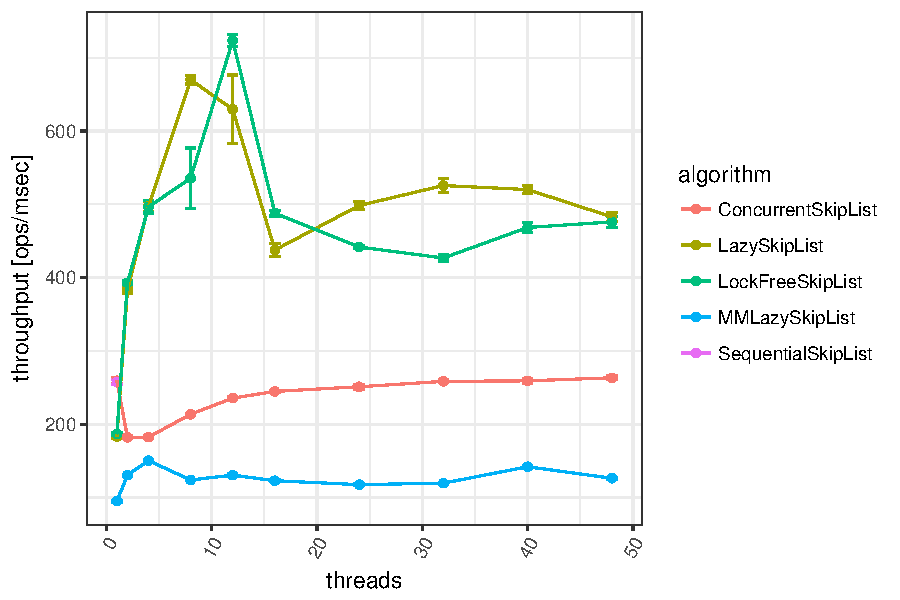
\includegraphics[width=\textwidth]{../plots/mixed_workload_-_50p_insert_,_20p_remove_,_30p_search_strong_0.pdf}
        \caption{50\% Insert, 20\% Remove, 30\% Contains}
        \label{fig:Scatter:OpenMPI:Rel:32}
    \end{subfigure}
    \begin{subfigure}[b]{0.49\textwidth}
        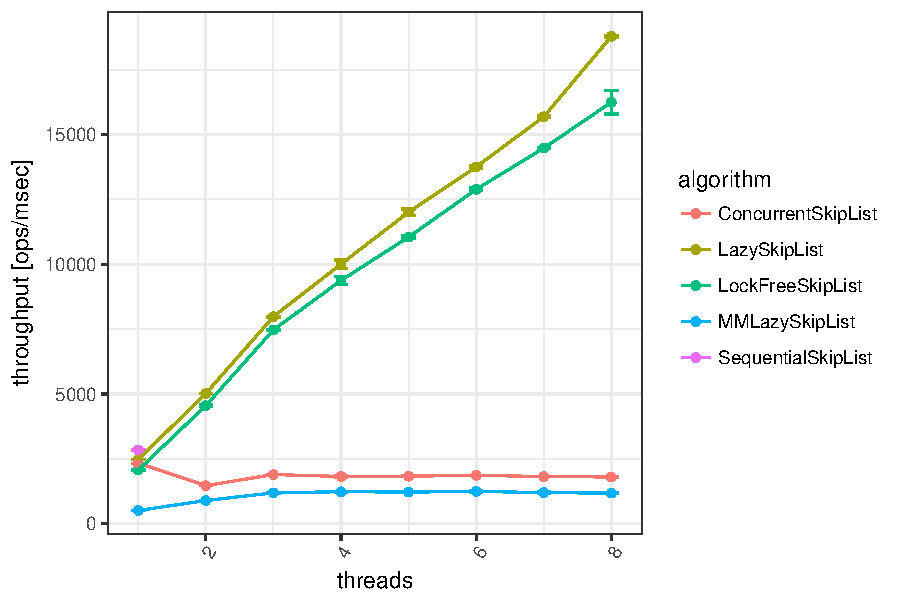
\includegraphics[width=\textwidth]{../plots/mixed_workload_-_70p_insert_,_30p_remove_strong_0.pdf}
        \caption{70\% Insert, 30\% Remove}
        \label{fig:Scatter:OpenMPI:Abs:32}
    \end{subfigure}
    
    \caption{SkipList throughput for different algorithms}
\end{figure}


\subsection{Performance Counters}

\begin{figure}[H]
    \centering
    
    \begin{subfigure}[b]{0.49\textwidth}
        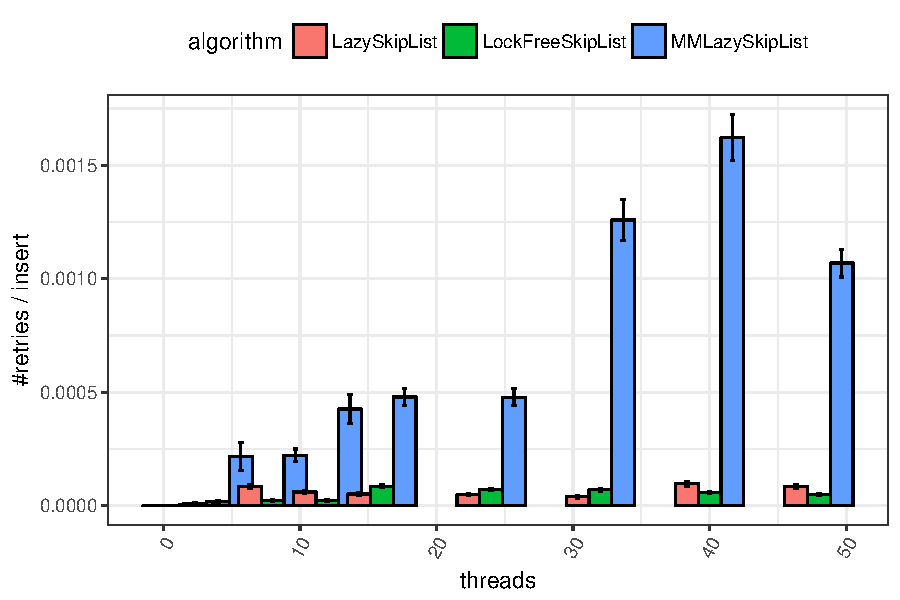
\includegraphics[width=\textwidth]{../plots/insert_retries_interleaving_insert_-_no_failed_inserts_strong_0.pdf}
        \caption{Interleaving Insert}
        \label{fig:Scatter:OpenMPI:Rel:31}
    \end{subfigure}
    \begin{subfigure}[b]{0.49\textwidth}
        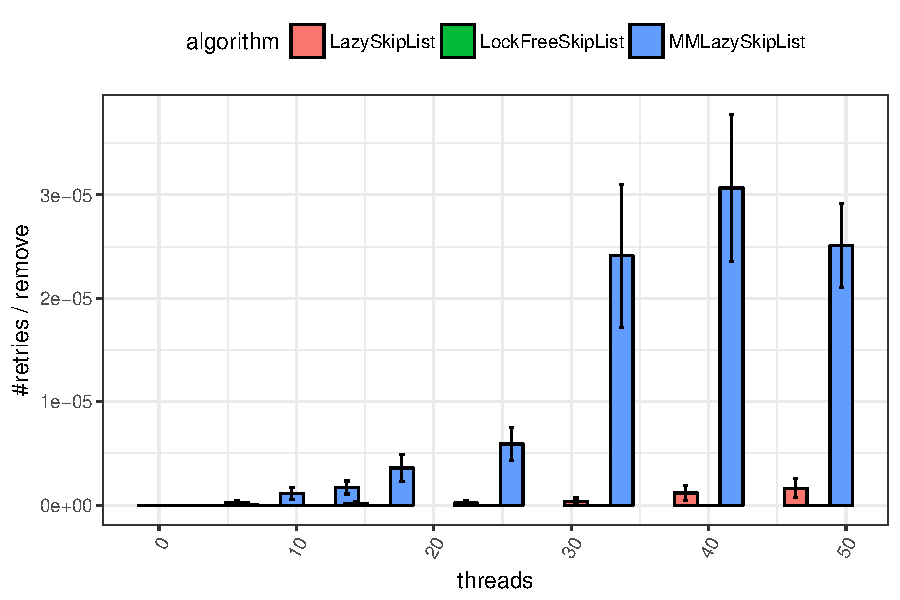
\includegraphics[width=\textwidth]{../plots/remove_retries_interleaving_remove_-_no_failed_removes_strong_0.pdf}
        \caption{Interleaving Remove}
        \label{fig:Scatter:OpenMPI:Abs:31}
    \end{subfigure}
    
    \begin{subfigure}[b]{0.49\textwidth}
        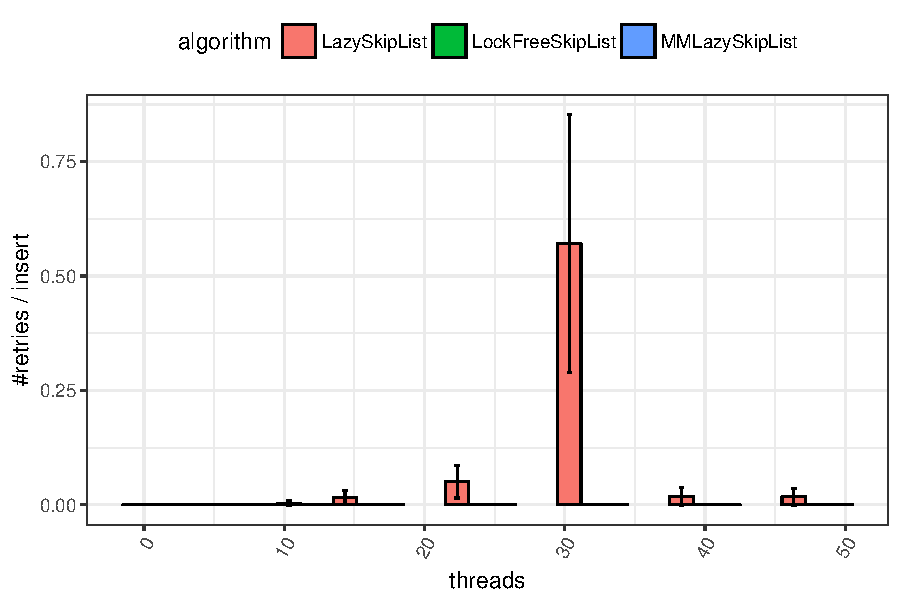
\includegraphics[width=\textwidth]{../plots/insert_retries_mixed_workload_-_50p_insert_,_20p_remove_,_30p_search_strong_0.pdf}
        \caption{50\% Insert, 20\% Remove, 30\% Contains}
        \label{fig:Scatter:OpenMPI:Rel:32}
    \end{subfigure}
    \begin{subfigure}[b]{0.49\textwidth}
        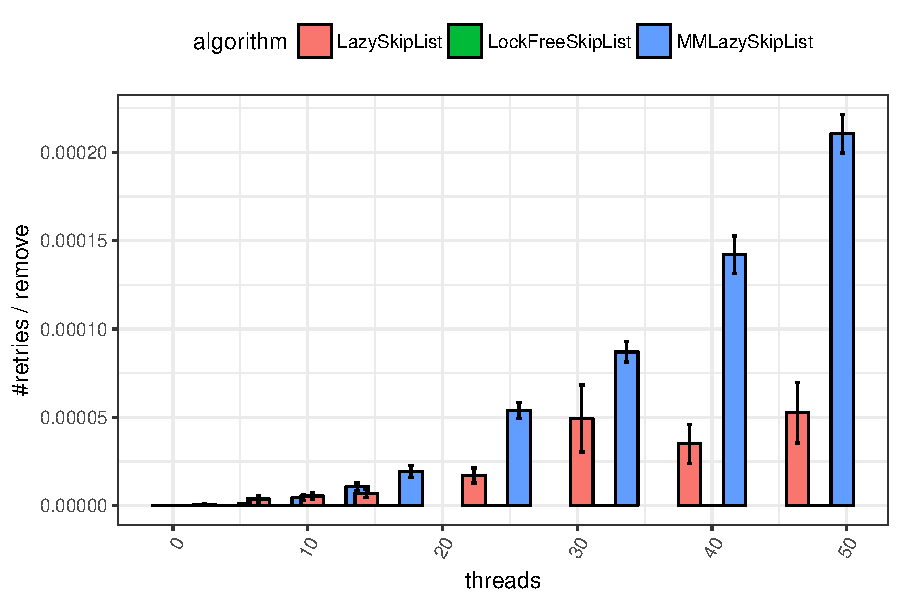
\includegraphics[width=\textwidth]{../plots/remove_retries_mixed_workload_-_70p_insert_,_30p_remove_strong_0.pdf}
        \caption{70\% Insert, 30\% Remove}
        \label{fig:Scatter:OpenMPI:Abs:32}
    \end{subfigure}
    
    \caption{Retries / Operation}
\end{figure}